%!TEX ROOT = thesis.tex
\chapter{THEORETICAL FRAMEWORK}
\label{chap: 3}

In this chapter we would start with a brief history of artificial intelligence research that are directly or indirectly related to the innovation of transformers. Then, the second section would covers the foundations of deep learning which includes feed-forward neural networks, activation functions, loss functions and evaluation metric. The  section would cover the basics of transformers. The final section would include the potential challenges and limitations of this project.

\section{A Brief History of Deep Learning}

Modern deep learning as we know it today can be traced back to when Frank Rosenblatt introduced the perceptron in 1959, referring to it as the "Mark I Perceptron" shown in figure \ref{fig:perceptron}. Given an input, the perceptron will generate an output based on a linear thresholding logic. The weights in the perceptron were updated and learned by iteratively reducing the difference between the generated output and the desired output and passing in a new input.

The perceptron never took off in popularity because Marvin Minsky and Seymour Papert showed the limitations of perceptrons in learning the simple XOR function. In 1986, David Rumelhart, Geoff Hinton, and Ronald Williams showed how by incorporating "hidden" layers, a multi-layer perceptron can be used to overcome the weakness of perceptrons in learning complex patterns. Multi-layer perceptrons are also known as neural networks.

\begin{figure}[ht]
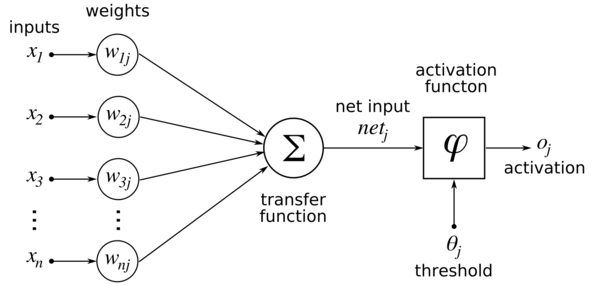
\includegraphics[width=10.5cm, height=5.5cm]{images/Rosenblattperceptron.png}
\centering
\caption{Rosenblatt Perceptron \protect\cite{markovbook}}
\label{fig:perceptron}
\end{figure}

LeCun et al., published a method to recognized hand-written digits and it was utilized by the U.S. Postal Service \cite{LeCunBoserDenkerEtAl89}, making it the first neural network model that received widesread adoption . This is a huge milestone for deep learning, proving the usefulness of convolution operations and weight learning the features in computer vision.

However, there are still a lot of flaws with neural networks. Take for example the backpropagation algorithm, has a number of issues such as vanishing gradients, exploding gradients, and the inability to learn long-term information. Hochreiter and Schmidhuber showed how  Long short-term memory (LSTM) architecture could overcome shortcomings of backpropagation over time.

LeCun et al. also showed the advantages of deep learning through more complex neural networks architectures such as convolutional neural networks (CNNs), restricted Boltzmann machines (RBMs), and deep belief networks (DBNs). They also showed the importance of techniques such as unsupervised pre-training
with fine-tuning, thus inspiring the next wave of deep learning. Li et al.,  launched ImageNet, which was the most extensive collection of labelled images and highlighted the importance of robust dataset to train a deep learning model for computer vision task. 

Mikolov et al. and Graves proposed language models using Recurrent Neural Networks (RNN) and LSTM, which later became the building blocks for many natural language processing (NLP) architectures. Sequence-to-sequence framework became the core architecture for a wide range of NLP tasks. Bahdanau et al. proposed the attention mechanism to overcome the bottleneck issue with sequence-tosequence model. Attention mechanismplays a crucial role in subsequent evolution of Transformers.

In 2017, Transformers were formally introduced in the "Attention is All You Need" paper \cite{attention-is-all-you-need} and became the most popular architecture in NLP. In 2020, Vision Transformers \cite{16x16} introduced a method to adapt Transformers for computer vision by splitting the input image into patches and represent them as vectors.

\section{Introduction to Transformers}
This section would  lays out the various building blocks of transformers such as attention, multi-head attention, positional encodings, residual connections, and encoder-decoder architecture. Subsections \ref{subsection: encoder-decoder} and \ref{subsection: sequence} would give a brief introduction to Recurrent Neural Networks (RNN) and sequence-to-sequence model (seq2seq) and the subsequent subsections would explain why attention unit and Transformers are born from RNN and seq2seq. 
\subsection{Encoder-Decoder Architecture} \label{subsection: encoder-decoder}

Because Transformers has its origin in NLP that relies on sequential input, the use of encoder-decoder architecture as shown in \ref{fig:encoder-decoder} such as RNN is very common. The encoder module takes a variable-length sequence and converts it into a fixed-length output-state while the decoder module takes a fixed-length state and converts it back into a variable-length output \cite{attention}.
\begin{figure}[ht]
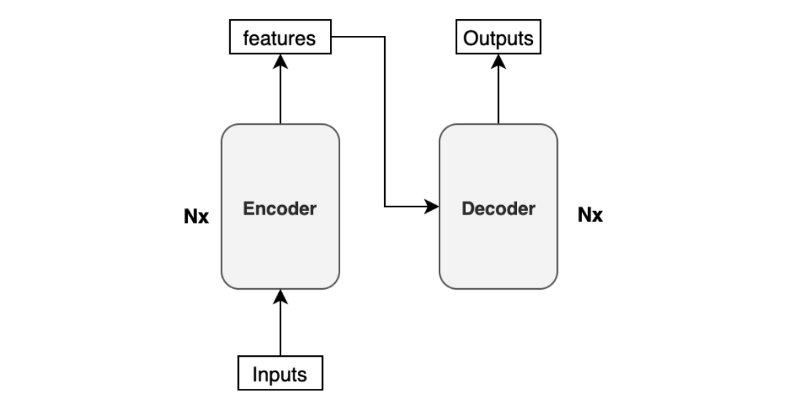
\includegraphics[width=13.5cm, height=5.5cm]{images/encodeer-decoder.jpg}
\centering
\caption{Encoder-Decoder Architecture \protect\cite{attention}}
\label{fig:encoder-decoder}
\end{figure}



\subsection{Sequence-To-Sequence} \label{subsection: sequence}

Sequence-to-sequence (seq2seq) is a type of deep learning approach where the input is in a sequence like a sentence and the context for each item is the output from the previous step. Seq2seq is the most famous model in Natural Language Processing. Suppose that we have an input sequence $x_1...x_t$, embedding mapping will transform the input sequence into vectors $\mathbf{x}_1...\mathbf{x}_t$. A unidirectional RNN at any time \textit{t} with a previous hidden state $\mathbf{h}_{t-1}$ and input $\mathbf{x}_t$ will generate a new hidden state:

\begin{equation}
    \mathbf{h}_t = tanh(\mathbf{Wh}_{t-1} + \mathbf{Wx}_t)
\end{equation}

The decoder has the output of the encoder and will generate the decoded output at each step. RNNs have issues with vanishing and explosive gradients. Also RNNs dependence on previous time
steps makes it very difficult to parallelize.

\subsection{Attention Mechanism}

Attention mechanism was first introduced by \cite{attention} and it is the most fundamental part of a Transformer which was introduced by Google in 2017 \cite{attention-is-all-you-need}. The attention unit will take input vectors $\mathbf{x}_1...\mathbf{x}_t$ to produce output vectors $\mathbf{y}_1...\mathbf{y}_t$. $\mathbf{y}_i$ is the weighted average of all the input vectors
\begin{equation}
    \mathbf{y}_i = \sum w_{ij}\mathbf{x}_j
\end{equation}
Where $w_{ij}$ is the dot product of $x_i$ and $x_j$. The dot product gives us a real numbered value so we apply a softmax function to map the values to [0,1] and to ensure that they sum to 1 over the entire sequence:
\begin{equation}
    w_{ij} = \frac{exp w_{ij}}{\sum_j exp w_{ij}}
\end{equation}
\subsection{Queries, Keys and Values}
Every input vector $\mathbf{x}_i$ is used in three different ways in the self attention operation:
\begin{enumerate}
    \item It is compared to every other vector to establish the weights for its own output $\mathbf{y}_i$
    \item It is compared to every other vector to establish the weights for the output of the j-th vector $\mathbf{y}_j$
    \item It is used as part of the weighted sum to compute each output vector once the weights have been established.

\end{enumerate}

These roles are called the \textbf{query}, \textbf{key} and \textbf{value}. Three new weight matrices are developed for each role namely: $\mathbf{W_q}, \mathbf{W_k}, \mathbf{W_v}$. These are the weights that are going to be learned by backpropagation which is going to be discussed in the next section. Since the average value of the dot product grows with the embedding dimension $d_k$, it helps to scale the dot product back a little to stop the inputs to the softmax function from growing too large.
  The attention mechanism can be formally described as:
\begin{equation}
\mathbf{Q} = \mathbf{W}_q \mathbf{x}_i
\end{equation}
\begin{equation}
    \mathbf{K} = \mathbf{W}_k \mathbf{x}_i
\end{equation}
\begin{equation}
    \mathbf{V} = \mathbf{W}_v \mathbf{x}_i 
\end{equation}
\begin{equation}
    ATTENTION(\mathbf{Q,K,V}) = softmax(\frac{\mathbf{Q} \mathbf{K}^T}{\sqrt{d_k}})\mathbf{V}
\end{equation}
\begin{equation}
    \mathbf{y} = \sum ATTENTION(\mathbf{Q,K,V})\mathbf{x}    
\end{equation}

Where $\mathbf{Q}$ is the query,  $\mathbf{K}$ is the key, $\mathbf{V}$ is the value, $\mathbf{d}_k$ is the number of heads and  $\mathbf{y}$ is the output vector. The attention mechanism is shown in figure \ref{fig:attention-unit}

\begin{figure}[ht]
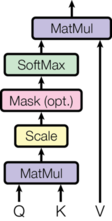
\includegraphics[width=4.0cm, height=6.5cm]{images/attention unit.png}
\centering
\caption{Illustration of Attention Mechanism Unit \protect\cite{attention-is-all-you-need}}
\label{fig:attention-unit}
\end{figure}
\FloatBarrier


\subsection{Multi Head Attention}

With the introduction of the softmax function in the previous section, we limit the attention value to either 0 or 1 when in reality attention can be anywhere in between. This is a negative consequence of using the softmax function. The easiest solution is to have multiple attention heads running at once. The multi-attention head is shown in figure \ref{fig:multi-head}.

\begin{figure}[ht]
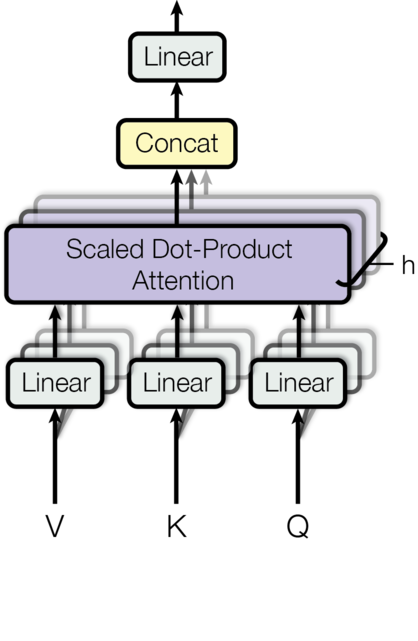
\includegraphics[width=5.5cm, height=7.5cm]{images/multi-head attention.png}
\centering
\caption{Illustration of Multi-head Attention \protect\cite{attention-is-all-you-need}}
\label{fig:multi-head}
\end{figure}
\FloatBarrier

Multi-attention head can be thought of as multiple copies of the self-attention mechanism running in parallel, each with their own key, value and query values. However, generating $\mathbf{K}$, $\mathbf{Q}$ and $\mathbf{V}$ for each head would be computationally expensive. We can avoid this problem by rescaling the weight matrix by dividing it with the square root of the number of heads and concatenating the $\mathbf{K}$, $\mathbf{Q}$ and $\mathbf{V}$ matrix as shown in \citeA{attention-is-all-you-need}. The entire Transformer architecture with multi-head attention head is shown in figure \ref{fig:transformer-architecture}

\begin{figure}[ht]
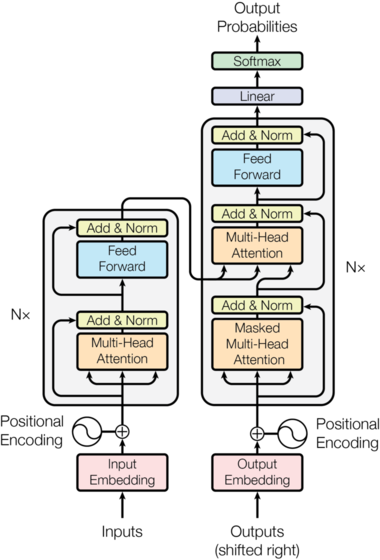
\includegraphics[width=6.5cm, height=9.5cm]{images/transformer_architecture.png}
\centering
\caption{Illustration of Transformer Architecture \protect\cite{attention-is-all-you-need}}
\label{fig:transformer-architecture}
\end{figure}
\FloatBarrier

\section{Activation Functions}
This section contains the three most commonly used asctivation functions in deep learning, namely the sigmoid function, the ReLU function and the softmax function.
\subsection{Sigmoid Function}
The sigmoid function is a special form of the logistic function and is given by:
\begin{equation}
    \sigma (x) = \frac{1}{1+exp(-x)}
\end{equation}

The sigmoid function would map any real numbered input to eaither 0 or 1. Figure \ref{fig: sigmoid} shows a plot of the sigmoid function.

\begin{figure}[ht]
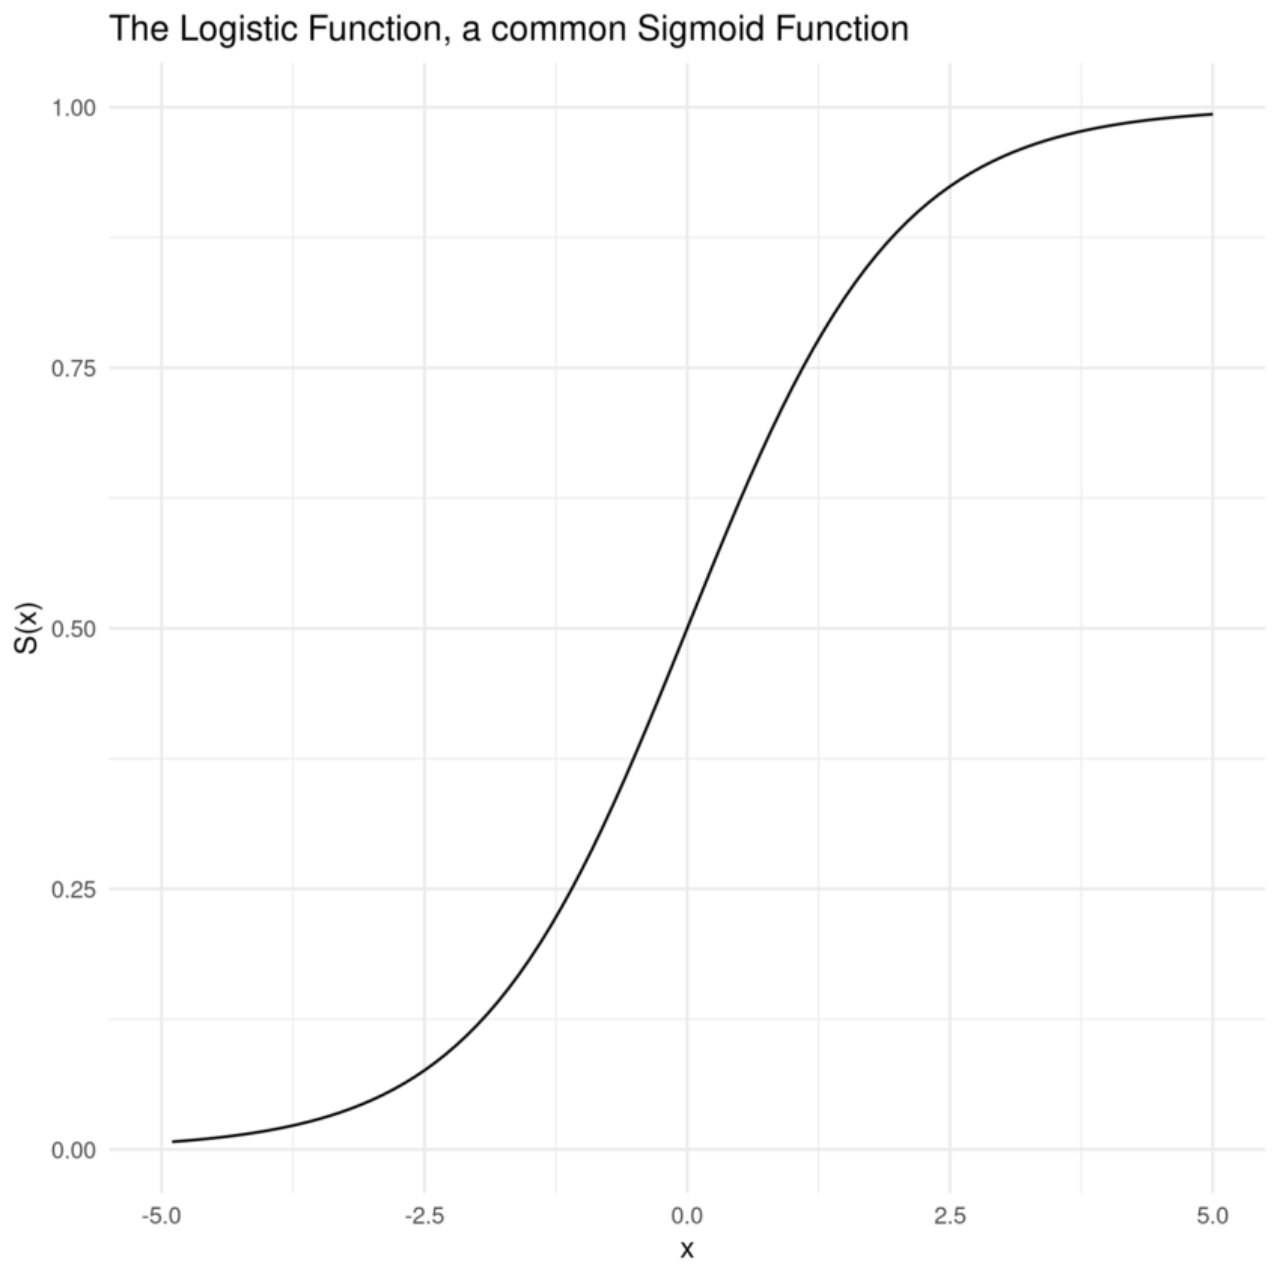
\includegraphics[width=7.5cm, height=6.5cm]{images/sigmoid.jpg}
\centering
\caption{Sigmoid Function}
\label{fig:sigmoid}
\end{figure}
\FloatBarrier


\subsection{Rectified Linear Unit Function}

There are several issues when we use sigmoid function for deep learning. The first issue is the function is only really sensitive to changes around its mid-point of its input. The second issue is that sigmoid function is computationally intensive. In order to use optimization technique such as SGD or ADAM with backpropagation  to train deep neural networks, we need a non-linear activation function that acts like a linear function. The function must also be more sensitive to changes in the input.

Rectified Linear Unit (ReLU) function returns the input value directly, or the value 0 if the input is 0 or less. Figure \ref{fig:relu} shows a plot of the ReLU function. ReLu function can be written as:
\begin{equation}
    f(x) = max(0,x)
\end{equation}

\begin{figure}[ht]
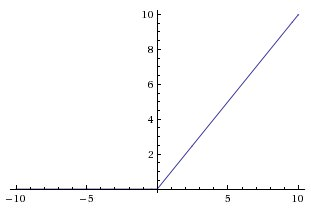
\includegraphics[width=7.5cm, height=6.5cm]{images/relu.jpeg}
\centering
\caption{ReLU Function}
\label{fig:relu}
\end{figure}
\FloatBarrier

\subsection{Softmax Function}

The softmax function is a function that takes a vector of K real values and ouput a vector of K real values that sum to 1. The input values can be any real numbers and softmax would map them into values between 0 and 1, so that they can be interpreted as probabilities. The softmax function is also known as the multi-class logistic regression and can be written as follows:
\begin{equation}
    \sigma(z) = \frac{e^{z_i}}{\sum_{j=1}^K e^{z_j}}
\end{equation}

where $z_i$ is an element of the input vector and the denominator is the sum of the input vector.

\section{Backpropagation}

The goal of backpropagation is to compute the partial derivative $\frac{\partial C}{\partial w}$ which is the partial derivative of $C$ with respect to weights and $\frac{\partial C}{\partial b}$ which is the partial derivative of $C$ with respect to bias. The cost function $C$ can be written as:
\begin{equation}
    C(X,\theta) = \frac{1}{2n} \sum_x ||\hat{y}(x) - y(x)||^2 
\end{equation}

where $n$ is the total number of training examples; the sum is over individual training examples, $x$; $\hat{y}(x)$ is the corresponding desired output; and y(x) is the vector of activations output from the network when $x$ is input.

In this example $C$ is the Euclidean distance between $y(x)$ and $a^L(x)$ which is a very common choice when training a neural network.Backpropagation attempts to minimize $C$ with respect to the neural network's weights by calculating, for each weight $w_{ij}^k$, the value of $\frac{\partial C}{\partial w_{ij}^k}$. At each iteration, the weights and biases (collectively denoted as $\theta$) is updated according to the learning rate, $\alpha$ as follows:
\begin{equation}
    \theta^{t+1} = \theta^t - \alpha \frac{\partial C(X,\theta^t)}{\partial \theta}
\end{equation}
where $\theta^t$ is the weights and biases of the neural network at iteration $t$ in gradient descent.

Since $C$ can be decomposed into a sum over individual error terms for each individual input-output pair, the derivative can be calculated with respect to each input-output pair individually and then combined at the end (since the derivative of a sum of functions is the sum of the derivatives of each function):
\begin{equation}
    \frac{\partial C(X,\theta)}{\partial w_{ij}^k} = \frac{1}{N} \sum_x \frac{\partial}{\partial w_{ij}^k}(\frac{1}{2}(\hat{y}_d-y_d)^2) = \frac{1}{N} \sum_x \frac{\partial C_d}{\partial w_{ij}^k}
\end{equation}

The derivation of the backpropagation algorithm begins by applying the chain rule to the partial derivative of $C$. Lastly, the weights are updated as follows:
\begin{equation}
    \Delta w_{ij}^k = - \alpha \frac{\partial C(X,\theta)}{\partial w_{ij}^k}
\end{equation}

\section{Potential Challenges and Limitations}

\begin{enumerate}
    \item \textbf{Weak Supervision}
        
        \cite{weakly-supervised-semantic} identified that a lot of semantic segmentation models doesn't work well under weak supervision. In this paper weak supervision is defined as using dataset that fulfil at least one of this criteria:
\begin{enumerate}
    \item \textit{Incomplete Supervision} - The dataset is small and insufficient to train a good model.
    \item \textit{Inexact supervision} - The labelling is not as exact as necessary which usually occurs in land cover labels with low resolution.
    \item \textit{Inaccurate supervision} - The labels are wrong.
\end{enumerate}
\item \textbf{Inadequate Computing Resource}
    
    Training a Vision Transformer model requires a lot of computation resource. Several papers took multiple days to train their model even though they are using multiple GPUs in parallel. 

\item \textbf{Large Model Size}

    The trained model would be quite large because we used a Transformer instead of CNN. A large model would take a long time to train and evaluate. Furthermore, it would also be harder to deploy it in the real world due to its size.

\end{enumerate}

